\subsection{Blobs}
En blob detektor finder regioner i billedet, der består af et sæt sammenhængnede pixels, alle af samme intensitet, der er distinktive ift. området. Lindenberg \cite{blob} definere blobs som værende lyse regioner på sort baggrund eller omvendt, altså strukturer, der står i kontrast til deres baggrund. En blob kan derfor defineres som et område med \emph{mindst} ét lokalt ekstrema, enten et maksima eller et minima. Det lokale ekstrema gør blobben til en veldefineret, lav-niveau struktur og derved interessant. Blobs har også en fordel ift. kant og hjørne detektion, da blobs indgår i de fleste domæner, hvor kanter og hjørner oftest forekommer i menneskeskabte scener, ved veldefinerede strukturer og har derfor flere applikationsområder.
\begin{figure}[H]
    \centering
    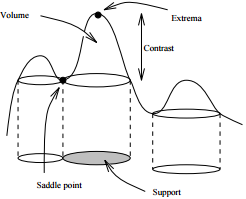
\includegraphics[width=0.35\textwidth]{fig/11.png}
    \vspace{-0.5em}   
    \begin{center}
    \caption{\textcolor{gray}{\footnotesize \textit{
    En blob visualiseret i 2-d, udefra Lindenberg's definition \cite{blob}}}}
    \label{fig:lindblob}
     \end{center}
  \end{figure}
       \vspace{-2.7em}
\noindent
I figur \ref{fig:lindblob}(a), ses en blob defineret af dets lokale ekstrema, hvor styrken af blobben beksrives ved kontrasten, ift. området omkring ekstremaet. Lindenberg definere blobbens domæne som værende afgrænset af dens "saddle point". Et "saddle point" angiver punktet, hvor intensiteten stopper med at falde og starter med at stige for lyse blobs, og modsat for mørke. Ligesom i kant-detektion, kan blobs beskrives ved intensitetsskift, hvor der forekommer en krusning rundt om ekstremaet. En metode til at detektere disse ekstremaer hedder Laplace operatoren $\Delta^2$, der er defineret som:
\begin{equation}
\Delta^2 f = \dfrac{\partial^2 f}{\partial x^2}+\dfrac{\partial^2 f}{\partial y^2}
\end{equation}
 Laplace operatoren anvendes på et gaussisk filter og kaldes 'Laplacian of Gaussian' forkortet: 'LoG' \eqref{lap}:
\begin{equation}
LoG=\sigma\Delta^2G
\label{lap}
\end{equation}
"LoG" operatoren kan diskritiseres og og foldes med billedet for at finde lokale ekstremaer. Figur \ref{fig:lapgauss} viser, hvordan laplace operatoren opnår et maximum i centeret af en blob, og at blobben derved bliver lokaliserbar. Hvis blobben (b), er tyndere eller tykkere vil laplace operatoren ikke længere resultere i et ekstrema, men nærmere en "bakke". Det er derfor nødvendigt at normalisere størrelsen af '$LoG$' filteret ift. hvilken størrelse blobben har.
\begin{figure}[H]
    \centering
    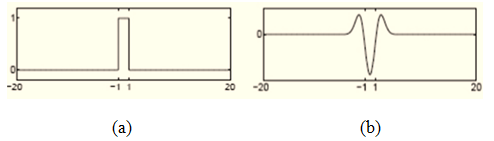
\includegraphics[width=0.60\textwidth]{fig/16.png}
    \vspace{-0.5em}   
    \begin{center}
    \caption{\textcolor{gray}{\footnotesize \textit{
    (a) En 3-D visualisering af en to-dimensional Laplacian of Guassian (b) ét en-dimensionalt signal (c) Laplacian of Gaussian operatoren anvendt på (b)}}}
    \label{fig:lapgauss}
     \end{center}
  \end{figure}
       \vspace{-2.5em}
\noindent
Blobs forekommer, ligesom andre strukturer, på forskellige skalaer, bestemt af størrelsen af objektet og objektets placering i billedet.
\begin{figure}[H]
    \centering
    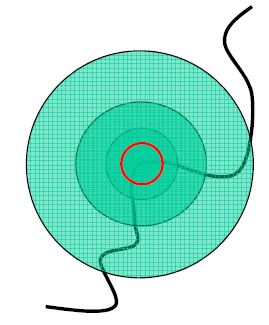
\includegraphics[width=0.25\textwidth]{fig/29.png}
    \vspace{-0.5em}   
    \begin{center}
    \caption{\textcolor{gray}{\footnotesize \textit{
    }}}
    \label{fig:scale}
     \end{center}
  \end{figure}
       \vspace{-2.5em}
\noindent
I figur \ref{fig:scale} angiver cirklerne forskellige undersøgte skalaer, Så hvordan udvælges cirklen, der dækker interesse området uafhængigt af områdets størrelse?  For Blobs er det interessant når der i et skaleret område opstår et veldefineret ekstrema. En måde at søge efter ekstremaer over forskellige skalaer er ved at oprette et skalarum for det undersøgte billede, hvor hvert billede skaleres og der for hver skala findes interessepunkter. Skala-rummet i et 2-dimensionalt billede repræsenteres af flere billeder i forskellige skalaer af det originale billede. Billeder, der repræsentere forskellige skalaer, opnås ved at folde billedet iterativt med et Gaussisk filter med stigende $\sigma$ værdi. 
\begin{figure}[H]
    \centering
    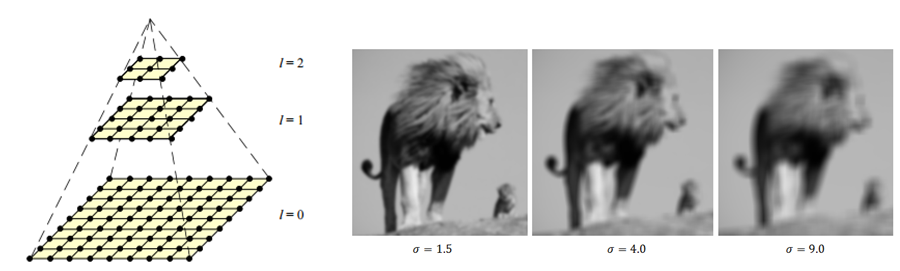
\includegraphics[width=0.65\textwidth]{fig/24.png}
    \vspace{-0.5em}   
    \begin{center}
    \caption{\textcolor{gray}{\footnotesize \textit{
Til venstre ses en visualisering af et skala-rum formet som en pyramide. Hvert niveau angiver en skala repræsentation af det originale vindue, hvor toppen af pyramiden indeholder billeder af største skala og derfor med mindst information, og bunden af skalaen med det originale billede. Til højre ses et billede foldet med et Gaussisk filter af stigende sigma værdier. Jo højere sigma værdi, jo flere fine detaljer bliver fjerne og billedet slørret.
    }}}
    \label{fig:mona}
     \end{center}
  \end{figure}
       \vspace{-2.5em}
\noindent
Et Gaussisk filter bruges da gradvis højere værdier af $\sigma$ fjerner fine strukturer, som vist i figur \ref{fig:mona}, og nye strukturer forekommer ikke ved transformationen fra finere til grovere skalaer \cite{lindenscale}. Idéen er derved at fjerne disse strukturer og lede efter  andre ekstremaer, gradvist på større skalaer, der også kan detekteres.
Et billede i skalarummet for billedet $f(x,y)$ kan derfor defineres som i \eqref{scalespace}
\begin{equation}
L(x,y,\sigma) = G(x,y,\sigma)\ast f(x,y)
\label{scalespace}
\end{equation}
hvor $G$ er det 2-dimensionelle Gaussiske filter,$L(x,y,\sigma)$ repræsentere et et billede i skala-rummet, og skala-parametren $\sigma$, bestemmer skalaen, eller placeringen i skala-rummet. $L(x,y,0) = f(x,y)$, da det er den "nederste" skala og den nederste del af pyramiden. Højere niveauer af pyramiden kan opnås ved at folde billedet med et Gaussisk filter af større sigma værdi.